% Use figure* for multi-column figure

\begin{figure}[tp]
  \centering

  \begin{subfigure}{0.45\textwidth}
    \centering
    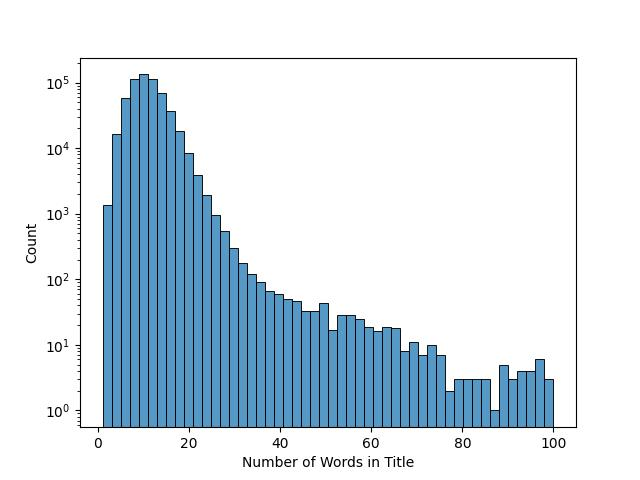
\includegraphics[width=\textwidth]{figs/data-statistic/title_lens.jpg}
    \caption{Title Length Distribution.}
    \label{fig:subfig1}
  \end{subfigure}
  \hfill
  \begin{subfigure}{0.45\textwidth}
    \centering
    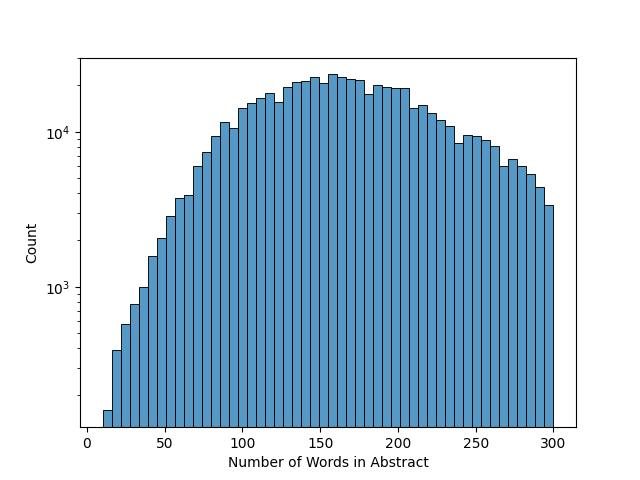
\includegraphics[width=\textwidth]{figs/data-statistic/abstract_lens.jpg}
    \caption{Abstract Length Distribution.}
    \label{fig:subfig2}
  \end{subfigure}

  \caption{Title and Abstract Statistic.}
  \label{fig:title-abstract-statistic}
\end{figure}